\documentclass{report}

\input{preamble}
\input{macros}
\input{letterfonts}

\title{\Huge{Abstract Algebra}}
\author{\huge{Rohan Jain}}
\date{}

\begin{document}

\maketitle
\newpage% or \cleardoublepage
% \pdfbookmark[<level>]{<title>}{<dest>}
\pdfbookmark[section]{\contentsname}{toc}
\tableofcontents

\pagebreak

\chapter{}
\section{Introductory Notes}

\subsection{Things to Remember}
\nt{
	\begin{itemize}
		\item Definitions will usually be stated as ``if" even though they mean ``if and only if".
		\item Any form of proof is valid. Avoid proofs by contradiction because of disbelief in the law of excluded middle.
		\item When you define an object, you can \emph{only} utilize its definition to prove anything about it.
	\end{itemize}
}

\subsection{Set Review}

\dfn{Set}{In mathematics, a set is an undefined term. Basically, ``everyone knows what it is.'' A few examples of sets are:

\begin{itemize}
	\item The empty set is the set with no elements. It is denoted by $\phi$ or $\emptyset$.
	\item $\NN$ is the set of natural numbers.
	\item $\ZZ$ is the set of integers.
	\item $\QQ$ is the set of rational numbers.
	\item $\RR$ is the set of real numbers.
	\item $\CC$ is the set of complex numbers.
\end{itemize}
}
\nt{
	\begin{itemize}
		\item A set is a well-defined collection of objects. The objects in a set are called elements of the set.
		\item A set is generally defined as a capital letter.
		\item $(A = B) \iff (\forall x : x \in A \iff x \in B)$
		\item $(A \subset B) \iff (\forall x \in A : x \in B)$
		\item $A$ is a proper subset of $B$ if $A \subset B$ and $A \neq B$.
	\end{itemize}
}

\thm{}{$A = B \iff A \subset B \land B \subset A$}

\nt{
	\begin{itemize}
		\item $A \cup B = {x:x\in A \lor x\in B}$
		\item $A \cap B = {x:x\in A \land x\in B}$
		\item $A$\textbackslash $B = {x:x\in A \land x\not\in B}$
		\item $C$\textbackslash $(A \cup B) = (C$\textbackslash $A) \cap (C$\textbackslash $B)$
	\end{itemize}
}

\subsection{Cartesian Products and Functions}
\nt{
	\begin{itemize}
		\item $A \times B = \{(a,b) : a \in A \land b \in B\}$
	\end{itemize}
}
\ex{Cartesian Product of two sets}{
	Let $A = \{1, 2, \Delta\}$ and $B = \{0, \pi\}$
	\begin{itemize}
		\item $(1, 0)$
		\item $(2, 0)$
		\item $(\Delta, 0)$
		\item $(1, \pi)$
		\item $(2, \pi)$
		\item $(\Delta, \pi)$
	\end{itemize}
}

\nt{Relations are subsets of Cartesian Products. For example, we can say that $<$ is a relation on the subset of $\RR \times \RR$ consisting of all ordered pairs of real numbers such that the first element is less than the second.}

\dfn{Function}{A function $f$ from a set $A$ to a set $B$ is a subset of $A \times B$ such that for every $a \in A$, there is exactly one $b \in B$ such that $(a, b) \in f$.}

\nt{Let $R$ be a relation from $A$ to $B$.
\begin{itemize}
	\item $A$ is the domain
	\item $B$ is the codomain
	\item $\{b: aRb\}$ is the image
	\item $R$ is injective (one-to-one) if $a_1Rb \land a_2Rb \implies a_1 = a_2$
	\item $R$ is surjective (onto) if $\forall b \in B : \exists a \in A : aRb$. Basically if the image is the entire codomain.
	\item $R$ is bijective if it is injective and surjective
\end{itemize}}

\nt{$A \xrightarrow{\text{R}} B$ \\ $B \xrightarrow{\text{S}} C$ \\ Define the composition as $S \circ R = \{(a, c) :$ there is some $b$ such that $(a, b) \in R$ and $(b, c) \in S$\} }

\thm{}{Let $f: A \to B$, $g: B \to C$, and $h: C \to D$. Then
\begin{itemize}
	\item $h \circ (g \circ f) = (h \circ g) \circ f$
	\item If $f$ and $g$ are injective, so is $g \circ f$
	\item If $f$ and $g$ are surjective, so is $g \circ f$
	\item If $f$ and $g$ are bijective, so is $g \circ f$
\end{itemize}}

\subsection{Equivalence Relations}
\dfn{Equivalence Relation}{An equivalence relation is a relation that has the following special properties:
\begin{itemize}
	\item Reflexivity: $aRa$ for all $a \in A$
	\item Symmetry: $aRb \implies bRa$
	\item Transitivity: $aRb \land bRc \implies aRc$
\end{itemize}}

\dfn{Partition}{Given a set $S$, a partition of $S$ is a collection of subsets of $S$ such that their union is $S$.}

\nt{Equivalence relations go hand in hand with partitions.}

\nt{If $\sim$ is an equivalence relation $a\sim b$, then $\sim$ partiations a set $X$ into chunks. $X / \sim$ is the set of chunks.

Addition is \emph{well-defined} as an operation on $\ZZ/x\ZZ$ for $x \in \ZZ$.}

\subsection{Complex Numbers and Matrices}
\dfn{Complex Number}{A complex number is a number of the form $a + bi$, where $a$ and $b$ are real numbers and $i$ is the imaginary unit. $i^2 = -1$.}

\nt{Complex numbers generally take the from $z = a + bi$. 

$\bar z = a - bi$ is the complex conjugate of $z$.}

\dfn{Matrix}{A matrix is a rectangular array of numbers.}

\subsection{Number Theory}


\section{Random Examples}
\clm{Topology}{}{Topology is cool}
\ex{Open Set and Close Set}{
	\begin{tabular}{rl}
		Open Set:   & $\bullet$ $\phi$                                              \\
		            & $\bullet$ $\bigcup\limits_{x\in X}B_r(x)$ (Any $r>0$ will do) \\[3mm]
		            & $\bullet$ $B_r(x)$ is open                                    \\
		Closed Set: & $\bullet$ $X,\ \phi$                                          \\
		            & $\bullet$ $\overline{B_r(x)}$                                 \\
		            & $x-$axis $\cup$ $y-$axis
	\end{tabular}}
\begin{myproof}By openness of $V$, $x\in B_r(u)\subset V$
	\begin{center}
		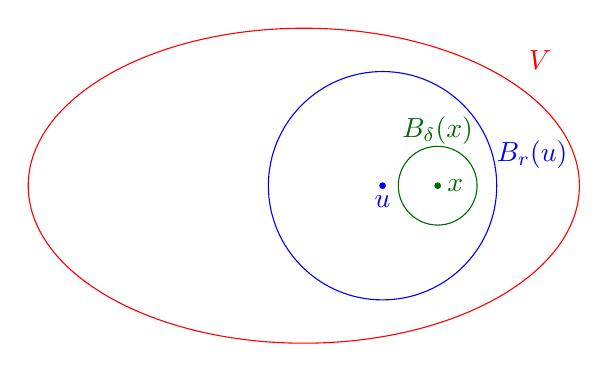
\begin{tikzpicture}
			\draw[red] (0,0) circle [x radius=3.5cm, y radius=2cm] ;
			\draw (3,1.6) node[red]{$V$};
			\draw [blue] (1,0) circle (1.45cm) ;
			\filldraw[blue] (1,0) circle (1pt) node[anchor=north]{$u$};
			\draw (2.9,0.4) node[blue]{$B_r(u)$};
			\draw [green!40!black] (1.7,0) circle (0.5cm) node [yshift=0.7cm]{$B_{\delta}(x)$} ;
			\filldraw[green!40!black] (1.7,0) circle (1pt) node[anchor=west]{$x$};
		\end{tikzpicture}
	\end{center}

	Given $x\in B_r(u)\subset V$, we want $\delta>0$ such that $x\in B_{\delta} (x)\subset B_r(u)\subset V$. Let $d=d(u,x)$. Choose $\delta $ such that $d+\delta<r$ (e.g. $\delta<\frac{r-d}{2}$)

	If $y\in B_{\delta}(x)$ we will be done by showing that $d(u,y)<r$ but $$d(u,y)\leq d(u,x)+d(x,y)<d+\delta<r$$
\end{myproof}

\cor{}{By the result of the proof, we can then show...}
\mlenma{}{Suppose $\vec{v_1}, \dots, \vec{v_n} \in \RR[n]$ is subspace of $\RR^n$.}
\mprop{}{$1 + 1 = 2$.}

\section{Random}
\dfn{Normed Linear Space and Norm $\boldsymbol{\|\cdot\|}$}{Let $V$ be a vector space over $\bbR$ (or $\bbC$). A norm on $V$ is function $\|\cdot\|\ V\to \bbR_{\geq 0}$ satisfying \begin{enumerate}[label=\bfseries\tiny\protect\circled{\small\arabic*}]
		\item \label{n:1}$\|x\|=0 \iff x=0$ $\forall$ $x\in V$
		\item \label{n:2}	$\|\lambda x\|=|\lambda|\|x\|$ $\forall$ $\lambda\in\bbR$(or $\bbC$), $x\in V$
		\item \label{n:3} $\|x+y\| \leq \|x\|+\|y\|$ $\forall$ $x,y\in V$ (Triangle Inequality/Subadditivity)
	\end{enumerate}And $V$ is called a normed linear space.

	$\bullet $ Same definition works with $V$ a vector space over $\bbC$ (again $\|\cdot\|\to\bbR_{\geq 0}$) where \ref{n:2} becomes $\|\lambda x\|=|\lambda|\|x\|$ $\forall$ $\lambda\in\bbC$, $x\in V$, where for $\lambda=a+ib$, $|\lambda|=\sqrt{a^2+b^2}$ }



\textbf{Special Case $\bs{p=1}$}: $\|x\|_1=|x_1|+|x_2|+\cdots+|x_m|$ is clearly a norm by usual triangle inequality. \par
\textbf{Special Case $\bs{p\to\infty\ (\bbR^m$ with $\|\cdot\|_{\infty})}$}: $\|x\|_{\infty}=\max\{|x_1|,|x_2|,\cdots,|x_m|\}$\\
For $m=1$ these $p-$norms are nothing but $|x|$.
Now exercise

\sol{\textbf{For Property \ref{n:3} for norm-2}	\subsubsection*{\textbf{When field is $\bbR:$}} We have to show\begin{align*}
		         & \sum_i(x_i+y_i)^2\leq \left(\sqrt{\sum_ix_i^2} +\sqrt{\sum_iy_i^2}\right)^2                                       \\
		\implies & \sum_i (x_i^2+2x_iy_i+y_i^2)\leq \sum_ix_i^2+2\sqrt{\left[\sum_ix_i^2\right]\left[\sum_iy_i^2\right]}+\sum_iy_i^2 \\
		\implies & \left[\sum_ix_iy_i\right]^2\leq \left[\sum_ix_i^2\right]\left[\sum_iy_i^2\right]
	\end{align*}So in other words prove $\langle x,y\rangle^2 \leq \langle x,x\rangle\langle y,y\rangle$ where
	$$\langle x,y\rangle =\sum\limits_i x_iy_i$$

	\begin{note}
		\begin{itemize}
			\item $\|x\|^2=\langle x,x\rangle$
			\item $\langle x,y\rangle=\langle y,x\rangle$
			\item $\langle \cdot,\cdot\rangle$ is $\bbR-$linear in each slot i.e. \begin{align*}
				      \langle rx+x',y\rangle=r\langle x,y\rangle+\langle x',y\rangle	\text{ and similarly for second slot}
			      \end{align*}Here in $\langle x,y\rangle$ $x$ is in first slot and $y$ is in second slot.
		\end{itemize}
	\end{note}Now the statement is just the Cauchy-Schwartz Inequality. For proof $$\langle x,y\rangle^2\leq \langle x,x\rangle\langle y,y\rangle $$ expand everything of $\langle x-\lambda y,x-\lambda y\rangle$ which is going to give a quadratic equation in variable $\lambda $ \begin{align*}
		\langle x-\lambda y,x-\lambda y\rangle & =\langle x,x-\lambda y\rangle-\lambda\langle y,x-\lambda y\rangle                                       \\
		                                       & =\langle x ,x\rangle -\lambda\langle x,y\rangle -\lambda\langle y,x\rangle +\lambda^2\langle y,y\rangle \\
		                                       & =\langle x,x\rangle -2\lambda\langle x,y\rangle+\lambda^2\langle y,y\rangle
	\end{align*}Now unless $x=\lambda y$ we have $\langle x-\lambda y,x-\lambda y\rangle>0$ Hence the quadratic equation has no root therefore the discriminant is greater than zero.

	\subsubsection*{\textbf{When field is $\bbC:$}}Modify the definition by $$\langle x,y\rangle=\sum_i\overline{x_i}y_i$$Then we still have $\langle x,x\rangle\geq 0$}

\section{Algorithms}
\begin{algorithm}[H]
\KwIn{This is some input}
\KwOut{This is some output}
\SetAlgoLined
\SetNoFillComment
\tcc{This is a comment}
\vspace{3mm}
some code here\;
$x \leftarrow 0$\;
$y \leftarrow 0$\;
\uIf{$ x > 5$} {
    x is greater than 5 \tcp*{This is also a comment}
}
\Else {
    x is less than or equal to 5\;
}
\ForEach{y in 0..5} {
    $y \leftarrow y + 1$\;
}
\For{$y$ in $0..5$} {
    $y \leftarrow y - 1$\;
}
\While{$x > 5$} {
    $x \leftarrow x - 1$\;
}
\Return Return something here\;
\caption{what}
\end{algorithm}

\end{document}